\begin{frame}{Communication protocols. $f: U \times V \to T$}
    \begin{center}
    	\onslide<1->{
    \tikzstyle{op1} = [opacity = 0]
    \tikzstyle{op2} = [opacity = 0]
    \tikzstyle{op3} = [opacity = 0]
    \tikzstyle{op4} = [opacity = 0]
}
\only<2->{\tikzstyle{op2} = [opacity = 1]}
\only<3->{\tikzstyle{op3} = [opacity = 1]}
\only<4->{\tikzstyle{op4} = [opacity = 1]}

\begin{tikzpicture}[black]
    \node[police, female, minimum size = 1.5cm] (alice) at (0, 0) {};
    \node[jester, mirrored, minimum size = 1.5cm] (bob) at (7, 0) {};
    \node[above = 0.3 of alice] {$x \in U$};
    \node[above = 0.3 of bob] {$y \in V$};

    \path (alice.east) -- (bob.west) node[midway, above = 2.3] {\Large $f(x, y) = ?$};
    \draw[op2, ->, thick] ($(alice.east) + (0.3, 1)$) -- ($(bob.west) + (-0.3, 1)$) node[midway, above] {$r_1 = a(x)$};
    \draw[op3, <-, thick] ($(alice.east) + (0.3, 0.2)$) -- ($(bob.west) + (-0.3, 0.2)$) node[midway, above] {$r_2 = b(y,
        r_1)$};
    \draw[op4, ->, thick] ($(alice.east) + (0.3, -0.2)$) -- ($(bob.west) + (-0.3, -0.2)$);
    \draw[op4, ->, thick] ($(alice.east) + (0.3, -0.6)$) -- ($(bob.west) + (-0.3, -0.6)$) node[midway, below] {$\vdots$};
\end{tikzpicture}    
    \end{center}

    \pause
    \pause
    \pause
	\pause
    
    The depth of the protocol is the number of rounds in the worst case.
    
    $CC(f) = \min\limits_{P \in \mathcal{P}} depth(P)$, where $\mathcal{P}$ is a set of protocols for $f$.
\end{frame}

\begin{frame}{Protocols and trees}

    Alice receives $u \in U$ and Bob receives $v \in V$. A communication protocols corresponds to a tree:

    \begin{columns}[t]
		\begin{column}{0.7\textwidth}
            \begin{itemize}
                \item<2-> inner vertices are marked by players;
	            \item<3-> if current player sends a bit they move to next vertex;
    		    \item<8-> leaves are marked by answers.
	        \end{itemize}

    		\onslide<9->{
                The size of the protocol is the size of the tree. $Size(f) = \min\limits_{P \in \mathcal{P}} size(P)$.
            } 
            \onslide<10->{
                \begin{lemma}[Kushilevitz, Nisan 1996]
                    $CC(f) = \Omega(\log(size(f)))$.
                \end{lemma}
            }
        \end{column}
        
		\begin{column}{0.25\textwidth}
            \tikzstyle{inner} = [thin, circle, minimum size = 0.3cm, draw, inner sep = 0.1pt, black]
\tikzstyle{inner_g} = [thin, circle, minimum size = 0.3cm, draw, inner sep = 0.1pt, black, fill = green]
\tikzstyle{inner_r} = [thin, circle, minimum size = 0.3cm, draw, inner sep = 0.1pt, black, fill = red]
\tikzstyle{inner_b} = [thin, circle, minimum size = 0.3cm, draw, inner sep = 0.1pt, black, fill = blue!50!white]
\tikzstyle{ed} = [thick, ->, draw, black]

    
\begin{tikzpicture}
    \only<-3, 5->{
        \node[inner] (a) at (0, 0) {\scriptsize $a$};
	}
    \only<4>{
        \node[inner_g] (a) at (0, 0) {\scriptsize $a$};
    }

    \only<-4, 6->{
        \node[inner] (b) at (-0.9, -1.2) {\scriptsize $b$};
	}
    \only<5>{
        \node[inner_g] (b) at (-0.9, -1.2) {\scriptsize $b$};
    }

    \node[inner] (c) at (0.9, -1.2) {\scriptsize $a$};
    \node[inner, label = below:$t_1$] (d) at (-1.5, -2.4) {};

    \only<-5, 7->{
        \node[inner] (e) at (-0.3, -2.4) {\scriptsize $b$};
	}
    \only<6>{
        \node[inner_g] (e) at (-0.3, -2.4) {\scriptsize $b$};
    }

    \node[inner] (e2) at (0.3, -2.4) {\scriptsize $b$};
    \node[inner, label = below:$t_4$] (f) at (1.5, -2.4) {};

    \only<-6, 9->{
        \node[inner, label = below:$t_2$] (g) at (-1.5, -4.3) {};
	}
    \only<7-8>{
        \node[inner_g, label = below:$t_2$] (g) at (-1.5, -4.3) {};
    }
    
    \node[inner, label = below:$t_3$] (h) at (-0.25, -4.3) {};
	\node[inner, label = below:$t_3$] (g2) at (1.5, -4.3) {};
    \node[inner, label = below:$t_2$] (h2) at (0.25, -4.3) {};
    
    \path (a) edge[ed] (b);
    \path (a) edge[ed] (c);
    \path (b) edge[ed] (d);
    \path (b) edge[ed] (e);
    \path (c) edge[ed] (e2);
    \path (c) edge[ed] (f);
    \path (e) edge[ed] (g);
    \path (e) edge[ed] (h);
    \path (e2) edge[ed] (g2);
    \path (e2) edge[ed] (h2);
\end{tikzpicture}

		\end{column}
	\end{columns}

\end{frame}


\begin{frame}{KW relation (Karchmer, Wigderson 1990)}
    A communication problem on sets $U, V \subseteq \{0, 1\}^{n}$ and relation $\Bit$:
    \begin{itemize}
        \item Alice receives $u \in U$, Bob receives $v \in V$;
        \item goal is to find $i$ such that $u_i \neq v_i$.
    \end{itemize}
    \pause
    Monotone case ($\MBit$ relation):
    \begin{itemize}
        \item goal is to find $i$ such that $u_i = 1 \land v_i = 0$.
    \end{itemize}

    \pause

    \begin{theorem}[Karchmer, Wigderson 1990]
        There is a \only<4->{\alert{(monotone)}} boolean {\color{blue} formula} for a function $f$ of the
        size $S$ iff there is a communication protocol of the size $S$ for the relation $\Bit$
        \only<4->{\alert{$(\MBit)$}}, $U = f^{-1}(1), V = f^{-1}(0)$.
    \end{theorem}

    \pause
    \pause
    
    \begin{theorem}[Pitassi, G{\"{o}}{\"{o}}s, 2014]
        There is a monotone function $f$ such that any monotone boolean formula that computes it has the
        size at least $2^{\frac{n}{\log(n)}}$. 
    \end{theorem}
\end{frame}


\begin{frame}{Canonical search problem $\Search_{\varphi}$ (Impagliazzo et al. 1994)}
    
    $\varphi(x, y)$ is an unsatisfiable CNF formula:
    \begin{itemize}
        \item Alice receives a substitution to the variables $x$, Bob receives a substitution to the
            variables $y$;
        \item goal is to find a clause $C \in \varphi$ that is unsatisfied by this substitution.
    \end{itemize}

    \pause

    \begin{theorem}[Beame, Pitassi, Segerlind 2007. Informal]
        If there is a {\color{blue} tree-like} proof in proof system $\Pi$ ($\Pi$ from some \textit{huge
          class}) of size $S$ then there is a communication protocol for $\Search_{\varphi}$ of depth
        $poly(\log(S))$.
    \end{theorem}

    \pause
    
    \begin{theorem}[Pitassi, G{\"{o}}{\"{o}}s, 2014]
        There is a formula $\varphi$ such that the communication complexity of $\Search_{\varphi}$ is at least
        $\frac{n}{\log(n)}$.
    \end{theorem}
\end{frame}

\begin{frame}{Generalization. Trivial way}

	\pause
    \begin{columns}[t]
		\begin{column}{0.6\textwidth}
            \onslide<2->{
                \begin{enumerate}
                    \item Structure of the protocol $\underset{\text{KW}}{\Leftrightarrow}$ structure of the formula.
                    \item Structure of the protocol $\underset{\text{IPU}}{\Leftarrow}$ structure of the proof.
                \end{enumerate}
            }
            
            \vspace{0.3cm}
            \onslide<3->{Can we merge some vertices in protocol?}

			\onslide<6->{
                \begin{block}{Remark}
                    It is too powerful model. There are short protocols for $\Bit$, $\MBit$ and
                    $\Search_{\varphi}$.
                \end{block}
            }
        \end{column}
        
		\begin{column}{0.25\textwidth}
            \tikzstyle{inner} = [thin, circle, minimum size = 0.3cm, draw, inner sep = 0.1pt, black]
\tikzstyle{inner_g} = [thin, circle, minimum size = 0.3cm, draw, inner sep = 0.1pt, black, fill = green]
\tikzstyle{inner_r} = [thin, circle, minimum size = 0.3cm, draw, inner sep = 0.1pt, black, fill = red]
\tikzstyle{inner_b} = [thin, circle, minimum size = 0.3cm, draw, inner sep = 0.1pt, black, fill = blue!50!white]
\tikzstyle{ed} = [thick, ->, draw, black]

    
\begin{tikzpicture}
    \only<-3, 5->{
        \node[inner] (a) at (0, 0) {\scriptsize $a$};
	}
    \only<4>{
        \node[inner_g] (a) at (0, 0) {\scriptsize $a$};
    }

    \only<-4, 6->{
        \node[inner] (b) at (-0.9, -1.2) {\scriptsize $b$};
	}
    \only<5>{
        \node[inner_g] (b) at (-0.9, -1.2) {\scriptsize $b$};
    }

    \node[inner] (c) at (0.9, -1.2) {\scriptsize $a$};
    \node[inner, label = below:$t_1$] (d) at (-1.5, -2.4) {};

    \only<-5, 7-10>{
        \node[inner] (e) at (-0.3, -2.4) {\scriptsize $b$};
	}
    \only<6>{
        \node[inner_g] (e) at (-0.3, -2.4) {\scriptsize $b$};
    }
    \only<11->{
        \node[inner_b] (e) at (-0.3, -2.4) {\scriptsize $b$};
    }

    \only<-10>{
        \node[inner] (e2) at (0.3, -2.4) {\scriptsize $b$};
	}
    \only<11>{
        \node[inner_b] (e2) at (0.3, -2.4) {\scriptsize $b$};
    }
    \only<12->{
        \node[inner_r] (e2) at (0.3, -2.4) {\scriptsize $b$};
    }
    
    \node[inner, label = below:$t_4$] (f) at (1.5, -2.4) {};

    \only<-6, 9->{
        \node[inner, label = below:$t_2$] (g) at (-1.5, -4.3) {};
	}
    \only<7-8>{
        \node[inner_g, label = below:$t_2$] (g) at (-1.5, -4.3) {};
    }
    
    \node[inner, label = below:$t_3$] (h) at (-0.25, -4.3) {};

    \only<-11>{
        \node[inner, label = below:$t_3$] (g2) at (1.5, -4.3) {};
	}
    \only<12->{
        \node[inner_r, label = below:$t_3$] (g2) at (1.5, -4.3) {};
    }

    \only<-11>{
        \node[inner, label = below:$t_2$] (h2) at (0.25, -4.3) {};
	}
    \only<12->{
        \node[inner_r, label = below:$t_2$] (h2) at (0.25, -4.3) {};
    }
    
    

    
    \path (a) edge[ed] (b);
    \path (a) edge[ed] (c);
    \path (b) edge[ed] (d);
    \path (b) edge[ed] (e);
    \only<-11>{
        \path (c) edge[ed] (e2);
    }
    \only<12->{
        \path (c) edge[ed] (e);
    }
    \path (c) edge[ed] (f);
    \path (e) edge[ed] (g);
    \path (e) edge[ed] (h);
    \path (e2) edge[ed] (g2);
    \path (e2) edge[ed] (h2);
\end{tikzpicture}

		\end{column}
	\end{columns}

\end{frame}

\begin{frame}{Properties of classical protocols}

    Fix any $u \in U$ and $v \in V$.

    \pause
    \begin{enumerate}
        \item Players can find ``next'' vertex in the tree in one round.
        \item For any vertex $h$ of the tree players can check whether they visit $h$ in one
            \textbf{parallel} round.
    \end{enumerate}

    \pause
    Relaxed version of second property:
    \begin{itemize}
        \item Some vertices of tree is marked by ``valid for (u, v)''.
        \item For any vertex $h$ of the tree players can check whether $h$ is valid for $(u, v)$ in one
            \textbf{parallel} round.
        \item If players start from valid vertex they find a correct answer.
    \end{itemize}
    
\end{frame}

\begin{frame}{Generalization. Rectangles}

    Alice receives $u \in U$ and Bob receives $v \in V$.

    \begin{columns}[t]
		\begin{column}{0.6\textwidth}
            \begin{itemize}
                \item<2-> Mark all vertices $h$ of the tree by rectangles $R_h = U_h \times V_h \subseteq
                    U \times V$;
	            \item<4-> $(u, v) \in R_h$ iff $h$ is on path from root to leaf for instance $(u, v)$;
    		    \item<6-> payment for merge $h$ and $h'$: cover by rectangle $R_{new}$.
	        \end{itemize}
            
            \onslide<5->{
                \begin{center}
                	\tikzstyle{end} = [thin, circle, minimum size = 0.1cm, draw, inner sep = 0.1pt]
\tikzstyle{leaf} = [thin, circle, minimum size = 0.6cm, draw, inner sep = 0.1pt, blue]
\tikzstyle{inner} = [thin, circle, minimum size = 0.2cm, draw, inner sep = 0.1pt, black]
            


\tikzstyle{ed} = [thick, ->, draw, black]

    
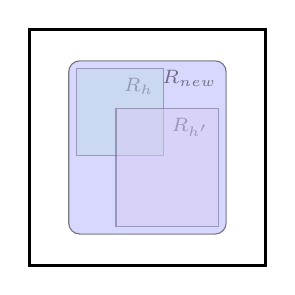
\begin{tikzpicture}[black]
    \draw[very thick] (0, 0) rectangle (3, 3);
    
    \draw[fill = green!20!white, opacity = 0.5] (0.6, 1.4) rectangle (1.7, 2.5) node[below left] {\scriptsize $R_{h}$};
    \draw[fill = red!10!white, opacity = 0.5] (1.1, 0.5) rectangle (2.4, 2.0) node[below left] {\scriptsize $R_{h'}$};

    \only<7->{
    	\draw[fill = blue!30!white, opacity = 0.5, rounded corners] (0.5, 0.4) rectangle (2.5, 2.6) node[below left]
	        {\scriptsize $R_{new}$};
    }
\end{tikzpicture}
    
                \end{center}
            }
        \end{column}
        
		\begin{column}{0.3\textwidth}
            \onslide<3->{\tikzstyle{inner} = [thin, circle, minimum size = 0.3cm, draw, inner sep = 0.1pt, black]
\tikzstyle{inner_g} = [thin, circle, minimum size = 0.3cm, draw, inner sep = 0.1pt, black, fill = green]
\tikzstyle{inner_r} = [thin, circle, minimum size = 0.3cm, draw, inner sep = 0.1pt, black, fill = red]
\tikzstyle{inner_b} = [thin, circle, minimum size = 0.3cm, draw, inner sep = 0.1pt, black, fill = blue!50!white]
\tikzstyle{ed} = [thick, ->, draw, black]

    
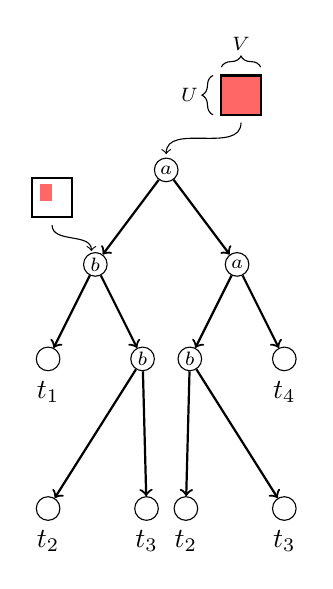
\begin{tikzpicture}
    \node[inner] (a) at (0, 0) {\scriptsize $a$};
    \node[inner] (b) at (-0.9, -1.2) {\scriptsize $b$};
    \node[inner] (c) at (0.9, -1.2) {\scriptsize $a$};
    \node[inner, label = below:$t_1$] (d) at (-1.5, -2.4) {};
    \node[inner] (e) at (-0.3, -2.4) {\scriptsize $b$};
    \node[inner] (e2) at (0.3, -2.4) {\scriptsize $b$};    
    \node[inner, label = below:$t_4$] (f) at (1.5, -2.4) {};
    \node[inner, label = below:$t_2$] (g) at (-1.5, -4.3) {};
    \node[inner, label = below:$t_3$] (h) at (-0.25, -4.3) {};
    \node[inner, label = below:$t_3$] (g2) at (1.5, -4.3) {};
    \node[inner, label = below:$t_2$] (h2) at (0.25, -4.3) {};

    
    \path (a) edge[ed] (b);
    \path (a) edge[ed] (c);
    \path (b) edge[ed] (d);
    \path (b) edge[ed] (e);
    \path (c) edge[ed] (e2);
    \path (c) edge[ed] (f);
    \path (e) edge[ed] (g);
    \path (e) edge[ed] (h);
    \path (e2) edge[ed] (g2);
    \path (e2) edge[ed] (h2);

    \draw[thick, black, fill = red!60!white] (0.7, 1.2) rectangle (1.2, 0.7);
    \draw [black, decorate, decoration = {brace, amplitude = 4pt}, xshift = -3pt] (0.7, 0.7) -- (0.7, 1.2)
	    node [black, midway, xshift = -0.3cm] {\scriptsize $U$};
    \draw [black, decorate, decoration = {brace, amplitude = 4pt}, yshift = 3pt] (0.7, 1.2) -- (1.2, 1.2)
    	node [black, midway, yshift = 0.3cm] {\scriptsize $V$};
    \draw[->] (0.95, 0.6) to[out = 270, in = 90] (0, 0.2);

    \draw[thick, black] (-1.7, -0.1) rectangle (-1.2, -0.6);
    \fill[red!60!white] (-1.6, -0.18) rectangle (-1.45, -0.4);
    \draw[->] (-1.45, -0.7) to[out = 270, in = 90] (-0.95, -1.03);
\end{tikzpicture}
}
		\end{column}
	\end{columns}
\end{frame}